\section{\ac{bus} images segmentation using optimization}\label{sec:methodApp}

This section defines the problem of delineating structures in \ac{bus} images as an optimization problem that can be solved applying the framework presented in Sect.\,{sec:method}.
In general terms, the image is divided in a discrete set $\mathcal{S}$, and each of these elements is associated with a label $l \in \{\text{lesion}, \overline{\text{lesion}}\}$ by simultaneously optimizing the data and pairwise terms. 

Figure~\ref{fig:methodterms} uses the problem of delineating the tissues present in a \ac{bus} images ($\mathcal{L} = \{ \text{chest wall}, \text{lungs}, \dots, \text{lesion} \}$) to illustrate the terms described in \cref{sec:method}. 

{\color{red}
In general, $\mathcal{S}$ can be any discrete set representing the image (i.e.\, pixels, overlapping or non overlapping windows, super-pixels, etc.). 
Figure~\ref{fig:methodTerms:problem} illustrates one such representation $\mathcal{S}$, applied to a \ac{bus} image example using super-pixels. The super-pixels are coloured according to the image's \ac{gt}.

Figure~\ref{fig:methodTerms:data} illustrates the data cost associated to some arbitrary labelling configurations to clarify the desired effect (or behaviour) of this data term (Fig.\,\ref{fig:methodTerms:problem} shows the \ac{gt} of each site $s$).
}

\begin{figure}
    \centering
    \begin{subfigure}[b]{0.19\textwidth}
        \centering
        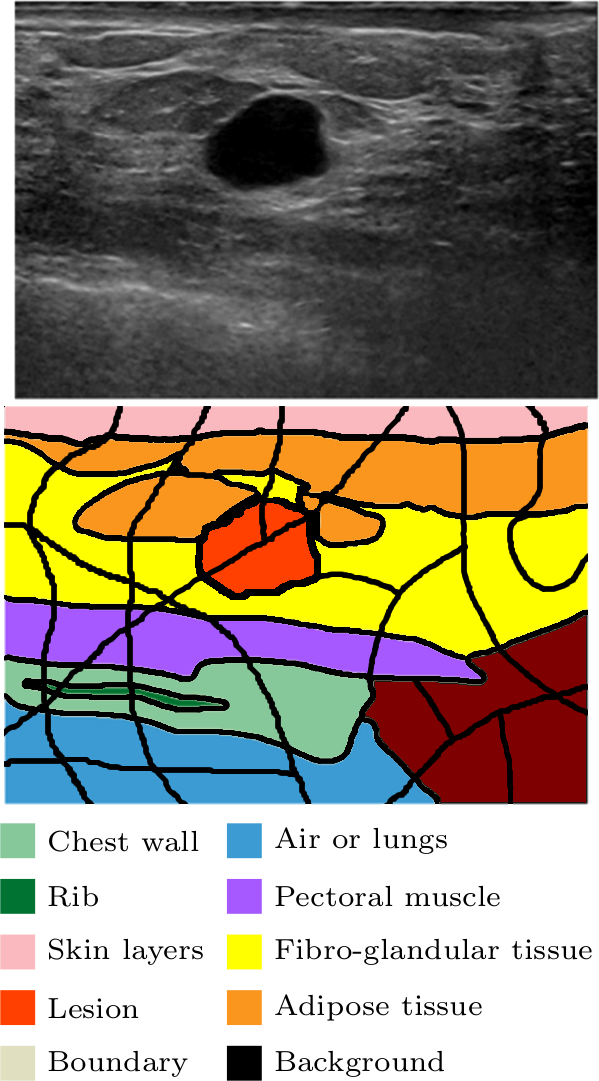
\includegraphics[width=\textwidth]{problem}
        %\caption{{\small Problem definition}}    
        \label{fig:methodTerms:problem}
    \end{subfigure}
    \hfill
    \begin{subfigure}[b]{0.39\textwidth}  
        \centering 
        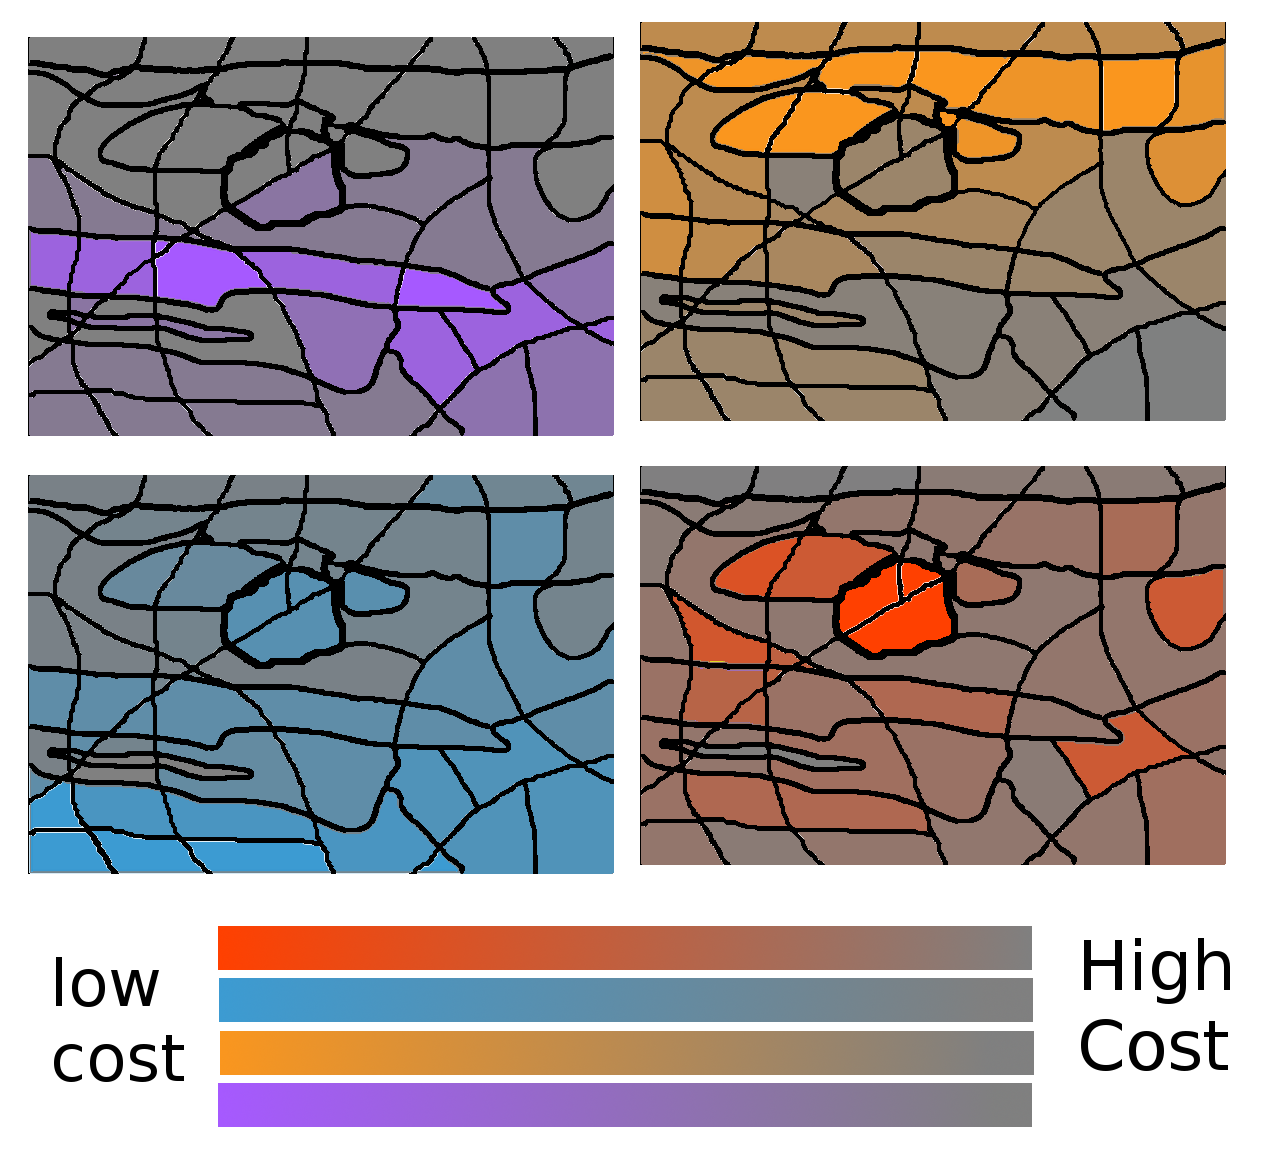
\includegraphics[width=\textwidth]{data}
        %\caption[]% {{\small Data term}}    
        \label{fig:methodTerms:data}
    \end{subfigure}
    \hfill
    \begin{subfigure}[b]{0.39\textwidth}   
        \centering 
        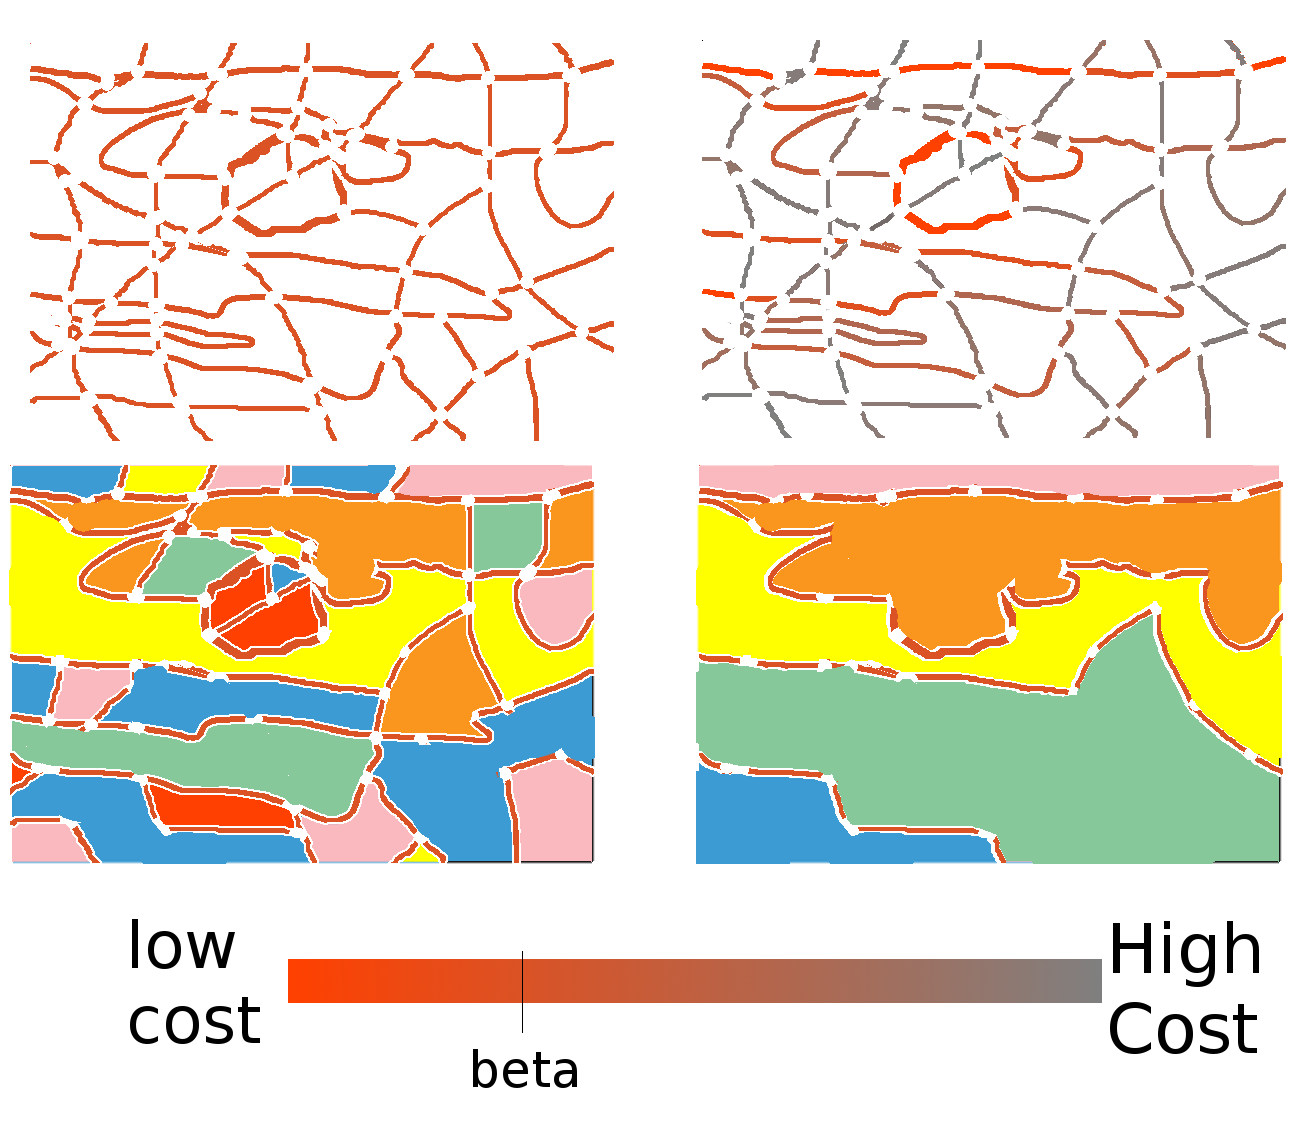
\includegraphics[width=\textwidth]{smooth} 
        %\caption[]% {{\small Pairwise term }}
        \label{fig:methodTerms:boundary}
    \end{subfigure}
    \caption {\small Methodology: (a) Problem definition, (b) Data term, (c) Pairwise term.} 
    \label{fig:methodterms}
\end{figure}


 We recall that the aim in segmentation is to affect to a discrete set of elements $\mathcal{S}$, a label $l$ from a labelling set $\mathcal{L}$. In our case, our labelling set $\mathcal{L} = \{ \text{chest wall}, \text{lungs}, \dots, \text{lesion} \}$ (see Fig\,\ref{fig:methodTerms:problem} for the entire set of labels) and the set $\mathcal{S}$ is chosen to be a super-pixels representation of the image~\cite{achanta2012slic}. In our case, $\mathcal{S}$ is the result from an over-segmentation of the image using Quick-shift super-pixel. Figure~\ref{fig:methodTerms:problem} illustrates one such representation $\mathcal{S}$, applied to a \ac{bus} image example. The super-pixels are coloured according to the image's \ac{gt}. Bear in mind that given an unseen \ac{bus} image, the ultimate goal is to represent the image as a set of super-pixels and infer the appropriated labelling for each of them.

\begin{figure}
  \includegraphics[width=0.9\textwidth]{lexiconReworked}
    \caption {{\footnotesize Visual reference: (a) breast structures, (b) US BI-RADS lexicon, (c) encoded visual cues.}} 
    \label{fig:features}
\end{figure}

In this section, the generic framework presented in the previous section is applied to \ac{bus} imaging. We need to define our problem properly. We recall that the aim in segmentation is to affect to a discrete set of elements $\mathcal{S}$, a label $l$ from a labelling set $\mathcal{L}$. In our case, our labelling set $\mathcal{L} = \{ \text{chest wall}, \text{lungs}, \dots, \text{lesion} \}$ (see Fig\,\ref{fig:methodTerms:problem} for the entire set of labels).

As illustrated in Fig.\,{\color{red}??}, choices have to be made regarding the different elements: the set $\mathcal{S}$, the data term $D(\cdot)$, the pairwise term $V(.)$, and the optimizer choice. These preferences are summarized in Table~{\color{red}??} and justified thereafter.

$\mathcal{S}$ is chosen to be the result from an over-segmentation of the input image using the Quick-shift super-pixel. The structures of the breast and their rendering when using a hand-held 2D \ac{us} probe are sketched in Fig.\,\ref{fig:features}. Figure~\ref{fig:features:lexicon} illustrates the lexicon proposed by the \ac{acr}~\cite{biradsus} and used by clinicians to perform their diagnosis. Thus, our aim is to generate a set of computer vision features which is able to encode the characteristic described in the lexicon. The selected features are the following:

\begin{description}
  \item[Appearance] 
    Based on the multi-labelled \ac{gt}, a \ac{mad} histogram model for every tissue label is built. The Appearance feature is computed as the $\chi^2$ distance between a histogram of $s$ and the models generated.
  \item[Atlas] 
    Based on the multi-labelled \ac{gt} an atlas is build to encode the labels likelihood based on the location of $s$.
  \item[Brightness] 
    Intensity descriptors are computed based on statistics of $s$ (\emph{i.e:} mean, median, mode) and  are compared with some intensity markers of the set $\mathcal{S}$ such as the minimum intensity value, the maximum, its mean, etc.
  \item[\ac{sift}-\ac{bof}]
    $s$ is described as an histogram of visual words based on \ac{sift}~\cite{massich2014sift}. The dictionary is built with $36$ words.
\end{description}

The relationships between the lexicon and the descriptors previously described is depicted in Table~{\color{red}??}. More precisely, we highlight the corresponding elements of the lexicon which is encoded by each feature. A choice regarding the encoding of the data term $D(\cdot)$ has to be made by using a \ac{ml} classifier. An \ac{svm} classifier with an \ac{rbf} kernel is selected to determine the data model during the training stage. The pairwise term is our framework was defined as in Eq.\,\eqref{eq:smoothing}. The optimization method used as solver to minimize our cost function $U(\cdot)$ is \ac{gc}. \ac{gc} when applicable allows to rapidly find a strong local minima guaranteeing that no other minimum with lower energies can be found~\cite{delong2012fast}. \ac{gc} is applicable if, and only if, the pairwise term favours coherent labelling configurations and penalizes labelling configurations where neighbours labels differs; such is our case, given by Eq.\,\eqref{eq:smoothing}.

%%% Local Variables: 
%%% mode: latex
%%% TeX-master: "../../master"
%%% End: 
